
\chapter{Presentation of the subject}

After this bibliographic study, I will present the subject of my work and the aim of it. My work supposed that a
model checking was done, so I will firstly explain that.

\section{Model checking}

Since few years, we are able to realize model to represent systems. These models permit to simulate systems. To do
these models, there is many languages UML, SysML, Fiacre,\dots The figure \ref{fig:model} represents an example of
a complex system.

\begin{figure}[h]
  \centering
  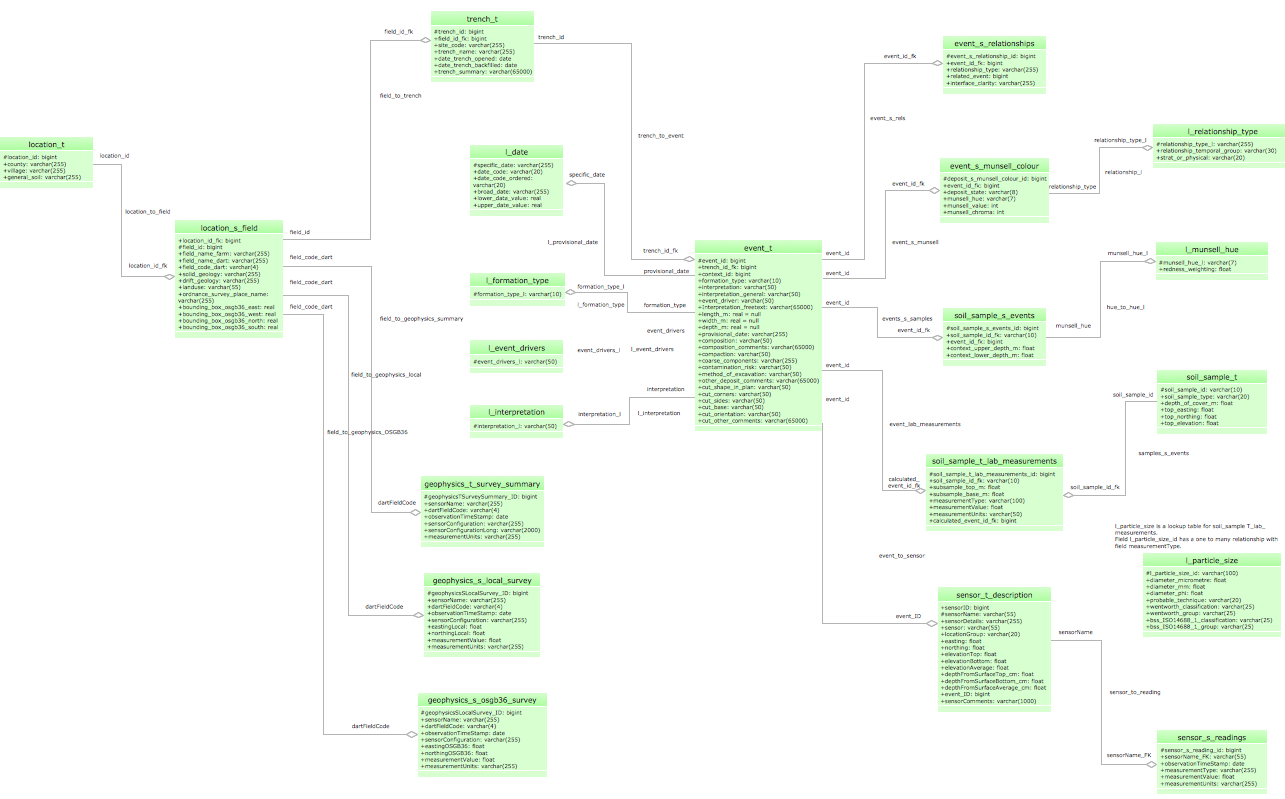
\includegraphics[width=\textwidth]{complex_model}
  \caption{Complex model in UML}
  \label{fig:model}
\end{figure}


Then with the simulation of these systems, we can imagine that we are able to find all possible states of our
system. So we know that if we are not in a valid state of the system, the system was potentially hacked.

\section{Position of my project}

So for my project, I guess I have all possible states for my system and I will check these possible states with the
current status of the system. To do so, I have to find the state of applications and the state of the network, and
analyze them.

I choose to use an IDS to have the status of the network. In fact, an IDS can raise alert when there is particular
message, so I will raise event when I sniff particular message. To have a status of an application, I choose to
implement probe in applications, or if it is possible use the log of these applications. Then, the SIEM will
correlate all these messages and alerts to find the status of our system and it will compare it with all previous
possible status.


The figure \ref{fig:model_project} represent the position of our project.

\begin{figure}[h]
  \centering
  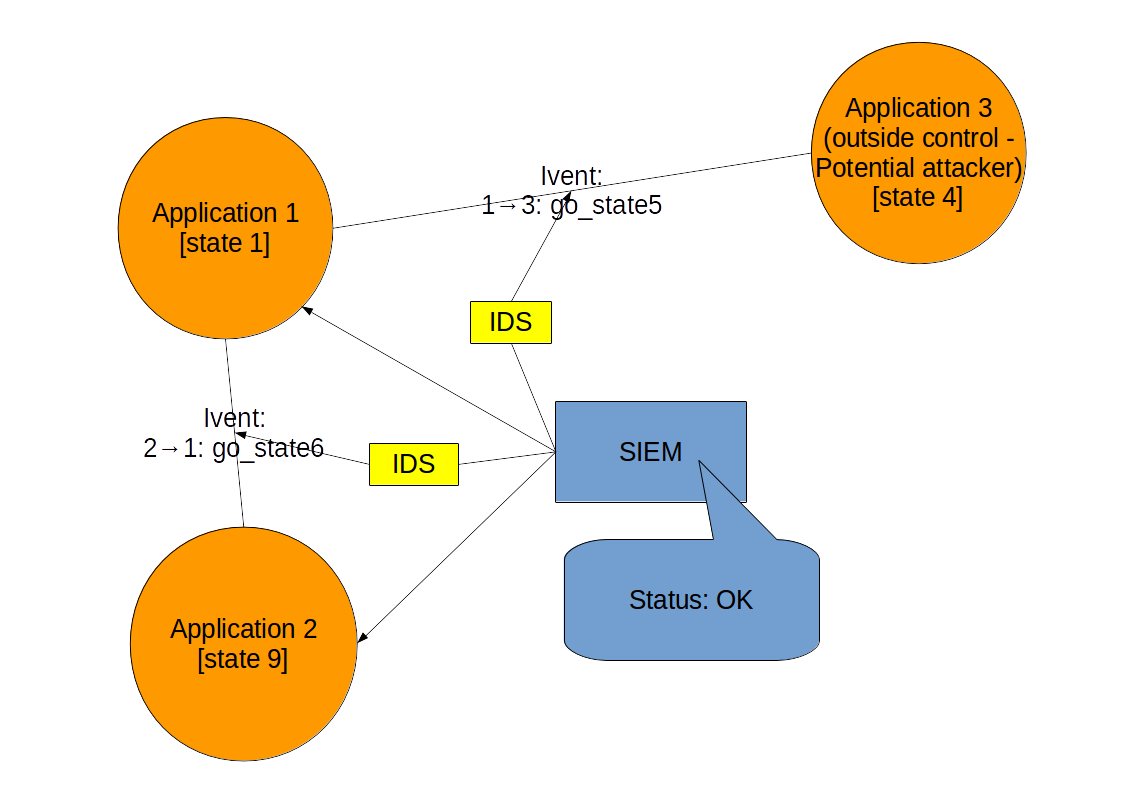
\includegraphics[width=\textwidth]{model_project}
  \caption{Position of my project}
  \label{fig:model_project}
\end{figure}




%%% Local Variables:
%%% mode: latex
%%% TeX-master: "../rapport_de_base"
%%% End:
